%%%%%%%%%%%%%%%%%%%%%%%%%%%%%%%%%%%%%%%%%
% Beamer Presentation
% LaTeX Template
% Version 2.0 (March 8, 2022)
%
% This template originates from:
% https://www.LaTeXTemplates.com
%
% Author:
% Vel (vel@latextemplates.com)
%
% License:
% CC BY-NC-SA 4.0 (https://creativecommons.org/licenses/by-nc-sa/4.0/)
%
%%%%%%%%%%%%%%%%%%%%%%%%%%%%%%%%%%%%%%%%%

%----------------------------------------------------------------------------------------
%	PACKAGES AND OTHER DOCUMENT CONFIGURATIONS
%----------------------------------------------------------------------------------------

\documentclass[
	14pt, % Set the default font size, options include: 8pt, 9pt, 10pt, 11pt, 12pt, 14pt, 17pt, 20pt
	%t, % Uncomment to vertically align all slide content to the top of the slide, rather than the default centered
	aspectratio=169, % Uncomment to set the aspect ratio to a 16:9 ratio which matches the aspect ratio of 1080p and 4K screens and projectors
]{beamer}
\usepackage[absolute,overlay]{textpos}
\usepackage{graphicx, makecell, setspace, tikz}
\usetikzlibrary{positioning,calc}

\graphicspath{{images/}{./}} % Specifies where to look for included images (trailing slash required)

\usepackage{booktabs} % Allows the use of \toprule, \midrule and \bottomrule for better rules in tables

%----------------------------------------------------------------------------------------
%	SET CHINESE FONT
%----------------------------------------------------------------------------------------

\usepackage{ctex}
\setCJKmainfont[BoldFont=STSong, ItalicFont=STKaiti]{STSong} % useless in beamer
\setCJKsansfont[BoldFont=STHeiti, ItalicFont=STKaiti]{STSong}
\setCJKmonofont{STFangsong}

%----------------------------------------------------------------------------------------
%	SET VARIABLE BLOCK
%----------------------------------------------------------------------------------------

\newenvironment<>{varblock}[2][1\textwidth]{%
  \setlength{\textwidth}{#1}
  \begin{actionenv}#3%
    \def\insertblocktitle{#2}%
    \par%
    \usebeamertemplate{block begin}}
  {\par%
    \usebeamertemplate{block end}%
  \end{actionenv}}
  
%----------------------------------------------------------------------------------------
%	SET LINE SPACING 
%----------------------------------------------------------------------------------------

\linespread{1.1} % Adjust line spacing

%----------------------------------------------------------------------------------------
%	SET FRAME TITLE
%----------------------------------------------------------------------------------------

\setlength{\parskip}{0.5ex}
\addtobeamertemplate{frametitle}{\vskip-0.9ex}{\vspace{0em}} % {}{adjust the height of frame title}{adjust the position of body paragraph}
%\setbeamertemplate{frametitle}{%
%    \nointerlineskip%
%    \begin{beamercolorbox}[wd=\paperwidth,ht=2.0ex,dp=0.6ex]{frametitle}
%        \hspace*{1ex}\insertframetitle%
%    \end{beamercolorbox}%
%}

%----------------------------------------------------------------------------------------
%	SELECT LAYOUT THEME
%----------------------------------------------------------------------------------------

% Beamer comes with a number of default layout themes which change the colors and layouts of slides. Below is a list of all themes available, uncomment each in turn to see what they look like.

%\usetheme{default}
%\usetheme{AnnArbor}
%\usetheme{Antibes}
%\usetheme{Bergen}
%\usetheme{Berkeley}
%\usetheme{Berlin}
%\usetheme{Boadilla}
%\usetheme{CambridgeUS}
%\usetheme{Copenhagen}
%\usetheme{Darmstadt}
%\usetheme{Dresden}
%\usetheme{Frankfurt}
%\usetheme{Goettingen}
%\usetheme{Hannover}
%\usetheme{Ilmenau}
%\usetheme{JuanLesPins}
%\usetheme{Luebeck}
\usetheme{Madrid}
%\usetheme{Malmoe}
%\usetheme{Marburg}
%\usetheme{Montpellier}
%\usetheme{PaloAlto}
%\usetheme{Pittsburgh}
%\usetheme{Rochester}
%\usetheme{Singapore}
%\usetheme{Szeged}
%\usetheme{Warsaw}

%----------------------------------------------------------------------------------------
%	SELECT COLOR THEME
%----------------------------------------------------------------------------------------

% Beamer comes with a number of color themes that can be applied to any layout theme to change its colors. Uncomment each of these in turn to see how they change the colors of your selected layout theme.

%\usecolortheme{albatross}
%\usecolortheme{beaver}
%\usecolortheme{beetle}
%\usecolortheme{crane}
%\usecolortheme{dolphin}
%\usecolortheme{dove}
%\usecolortheme{fly}
%\usecolortheme{lily}
%\usecolortheme{monarca}
%\usecolortheme{seagull}
%\usecolortheme{seahorse}
%\usecolortheme{spruce}
%\usecolortheme{whale}
%\usecolortheme{wolverine}

%----------------------------------------------------------------------------------------
%	SELECT FONT THEME & FONTS
%----------------------------------------------------------------------------------------

% Beamer comes with several font themes to easily change the fonts used in various parts of the presentation. Review the comments beside each one to decide if you would like to use it. Note that additional options can be specified for several of these font themes, consult the beamer documentation for more information.

\usefonttheme{default} % Typeset using the default sans serif font
%\usefonttheme{serif} % Typeset using the default serif font (make sure a sans font isn't being set as the default font if you use this option!)
%\usefonttheme{structurebold} % Typeset important structure text (titles, headlines, footlines, sidebar, etc) in bold
%\usefonttheme{structureitalicserif} % Typeset important structure text (titles, headlines, footlines, sidebar, etc) in italic serif
%\usefonttheme{structuresmallcapsserif} % Typeset important structure text (titles, headlines, footlines, sidebar, etc) in small caps serif

%------------------------------------------------

%\usepackage{mathptmx} % Use the Times font for serif text
\usepackage{palatino} % Use the Palatino font for serif text

%\usepackage{helvet} % Use the Helvetica font for sans serif text
\usepackage[default]{opensans} % Use the Open Sans font for sans serif text
%\usepackage[default]{FiraSans} % Use the Fira Sans font for sans serif text
%\usepackage[default]{lato} % Use the Lato font for sans serif text

%----------------------------------------------------------------------------------------
%	SELECT INNER THEME
%----------------------------------------------------------------------------------------

% Inner themes change the styling of internal slide elements, for example: bullet points, blocks, bibliography entries, title pages, theorems, etc. Uncomment each theme in turn to see what changes it makes to your presentation.

%\useinnertheme{default}
\useinnertheme{circles}
%\useinnertheme{rectangles}
%\useinnertheme{rounded}
%\useinnertheme{inmargin}

%----------------------------------------------------------------------------------------
%	SELECT OUTER THEME
%----------------------------------------------------------------------------------------

% Outer themes change the overall layout of slides, such as: header and footer lines, sidebars and slide titles. Uncomment each theme in turn to see what changes it makes to your presentation.

%\useoutertheme{default}
%\useoutertheme{infolines}
%\useoutertheme{miniframes}
%\useoutertheme{smoothbars}
%\useoutertheme{sidebar}
%\useoutertheme{split}
%\useoutertheme{shadow}
%\useoutertheme{tree}
%\useoutertheme{smoothtree}

%\setbeamertemplate{footline} % Uncomment this line to remove the footer line in all slides
%\setbeamertemplate{footline}[page number] % Uncomment this line to replace the footer line in all slides with a simple slide count

%\setbeamertemplate{navigation symbols}{} % Uncomment this line to remove the navigation symbols from the bottom of all slides

%----------------------------------------------------------------------------------------
%	PRESENTATION INFORMATION
%----------------------------------------------------------------------------------------

\title[学位论文题目]{\textbf{学位论文题目}} % The short title in the optional parameter appears at the bottom of every slide, the full title in the main parameter is only on the title page

%\subtitle{Optional Subtitle} % Presentation subtitle, remove this command if a subtitle isn't required

\author[姓名]{姓名} % Presenter name(s), the optional parameter can contain a shortened version to appear on the bottom of every slide, while the main parameter will appear on the title slide

\institute[学校]{学校 \\ \smallskip \textit{xxx@xxx.edu.cn}} % Your institution, the optional parameter can be used for the institution shorthand and will appear on the bottom of every slide after author names, while the required parameter is used on the title slide and can include your email address or additional information on separate lines

\date[\today]{硕士学位论文答辩 \\ \today} % Presentation date or conference/meeting name, the optional parameter can contain a shortened version to appear on the bottom of every slide, while the required parameter value is output to the title slide

%----------------------------------------------------------------------------------------

\begin{document}

%----------------------------------------------------------------------------------------
%	TITLE SLIDE
%----------------------------------------------------------------------------------------

\begin{frame}
	\titlepage % Output the title slide, automatically created using the text entered in the PRESENTATION INFORMATION block above
\end{frame}

%----------------------------------------------------------------------------------------
%	TABLE OF CONTENTS SLIDE
%----------------------------------------------------------------------------------------

% The table of contents outputs the sections and subsections that appear in your presentation, specified with the standard \section and \subsection commands. You may either display all sections and subsections on one slide with \tableofcontents, or display each section at a time on subsequent slides with \tableofcontents[pausesections]. The latter is useful if you want to step through each section and mention what you will discuss.

\begin{frame}
	\frametitle{目录} % Slide title, remove this command for no title
	
	\tableofcontents % Output the table of contents (all sections on one slide)
	%\tableofcontents[pausesections] % Output the table of contents (break sections up across separate slides)
\end{frame}

%----------------------------------------------------------------------------------------
%	PRESENTATION BODY SLIDES
%----------------------------------------------------------------------------------------

\section{研究背景} % Sections are added in order to organize your presentation into discrete blocks, all sections and subsections are automatically output to the table of contents as an overview of the talk but NOT output in the presentation as separate slides

%------------------------------------------------

\begin{frame}
	\frametitle{研究背景}
	\begin{varblock}[0.55\textwidth]{}
		图像。
	\end{varblock}	
	\begin{varblock}[0.55\textwidth]{}
		其中。
	\end{varblock}	

	\begin{textblock*}{6cm}(9.5cm,2.5cm) % {block width} (coords)
		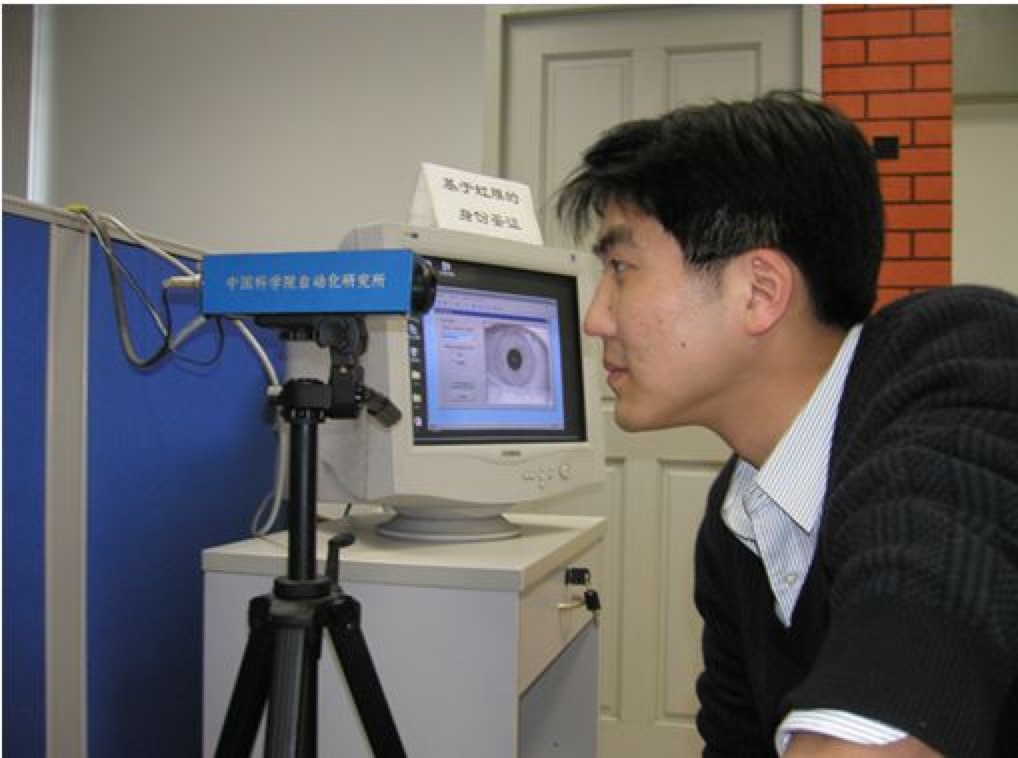
\includegraphics[width=6cm]{device.jpg}
	\end{textblock*}	

\end{frame}


%------------------------------------------------

\section{研究内容}

\subsection{方法1}

\subsubsection{理论分析}

%------------------------------------------------

\begin{frame}
	\frametitle{\large 方法1}
	\framesubtitle{\normalsize 骨干网络} % Optional subtitle
	\begin{varblock}[0.7\textwidth]{}
		现有的。
	\end{varblock}	
	\begin{varblock}[0.7\textwidth]{}
		本章提出了方法1,
	\end{varblock}	
	\begin{textblock*}{4.5cm}(11.3cm,1.8cm) % {block width} (coords)
		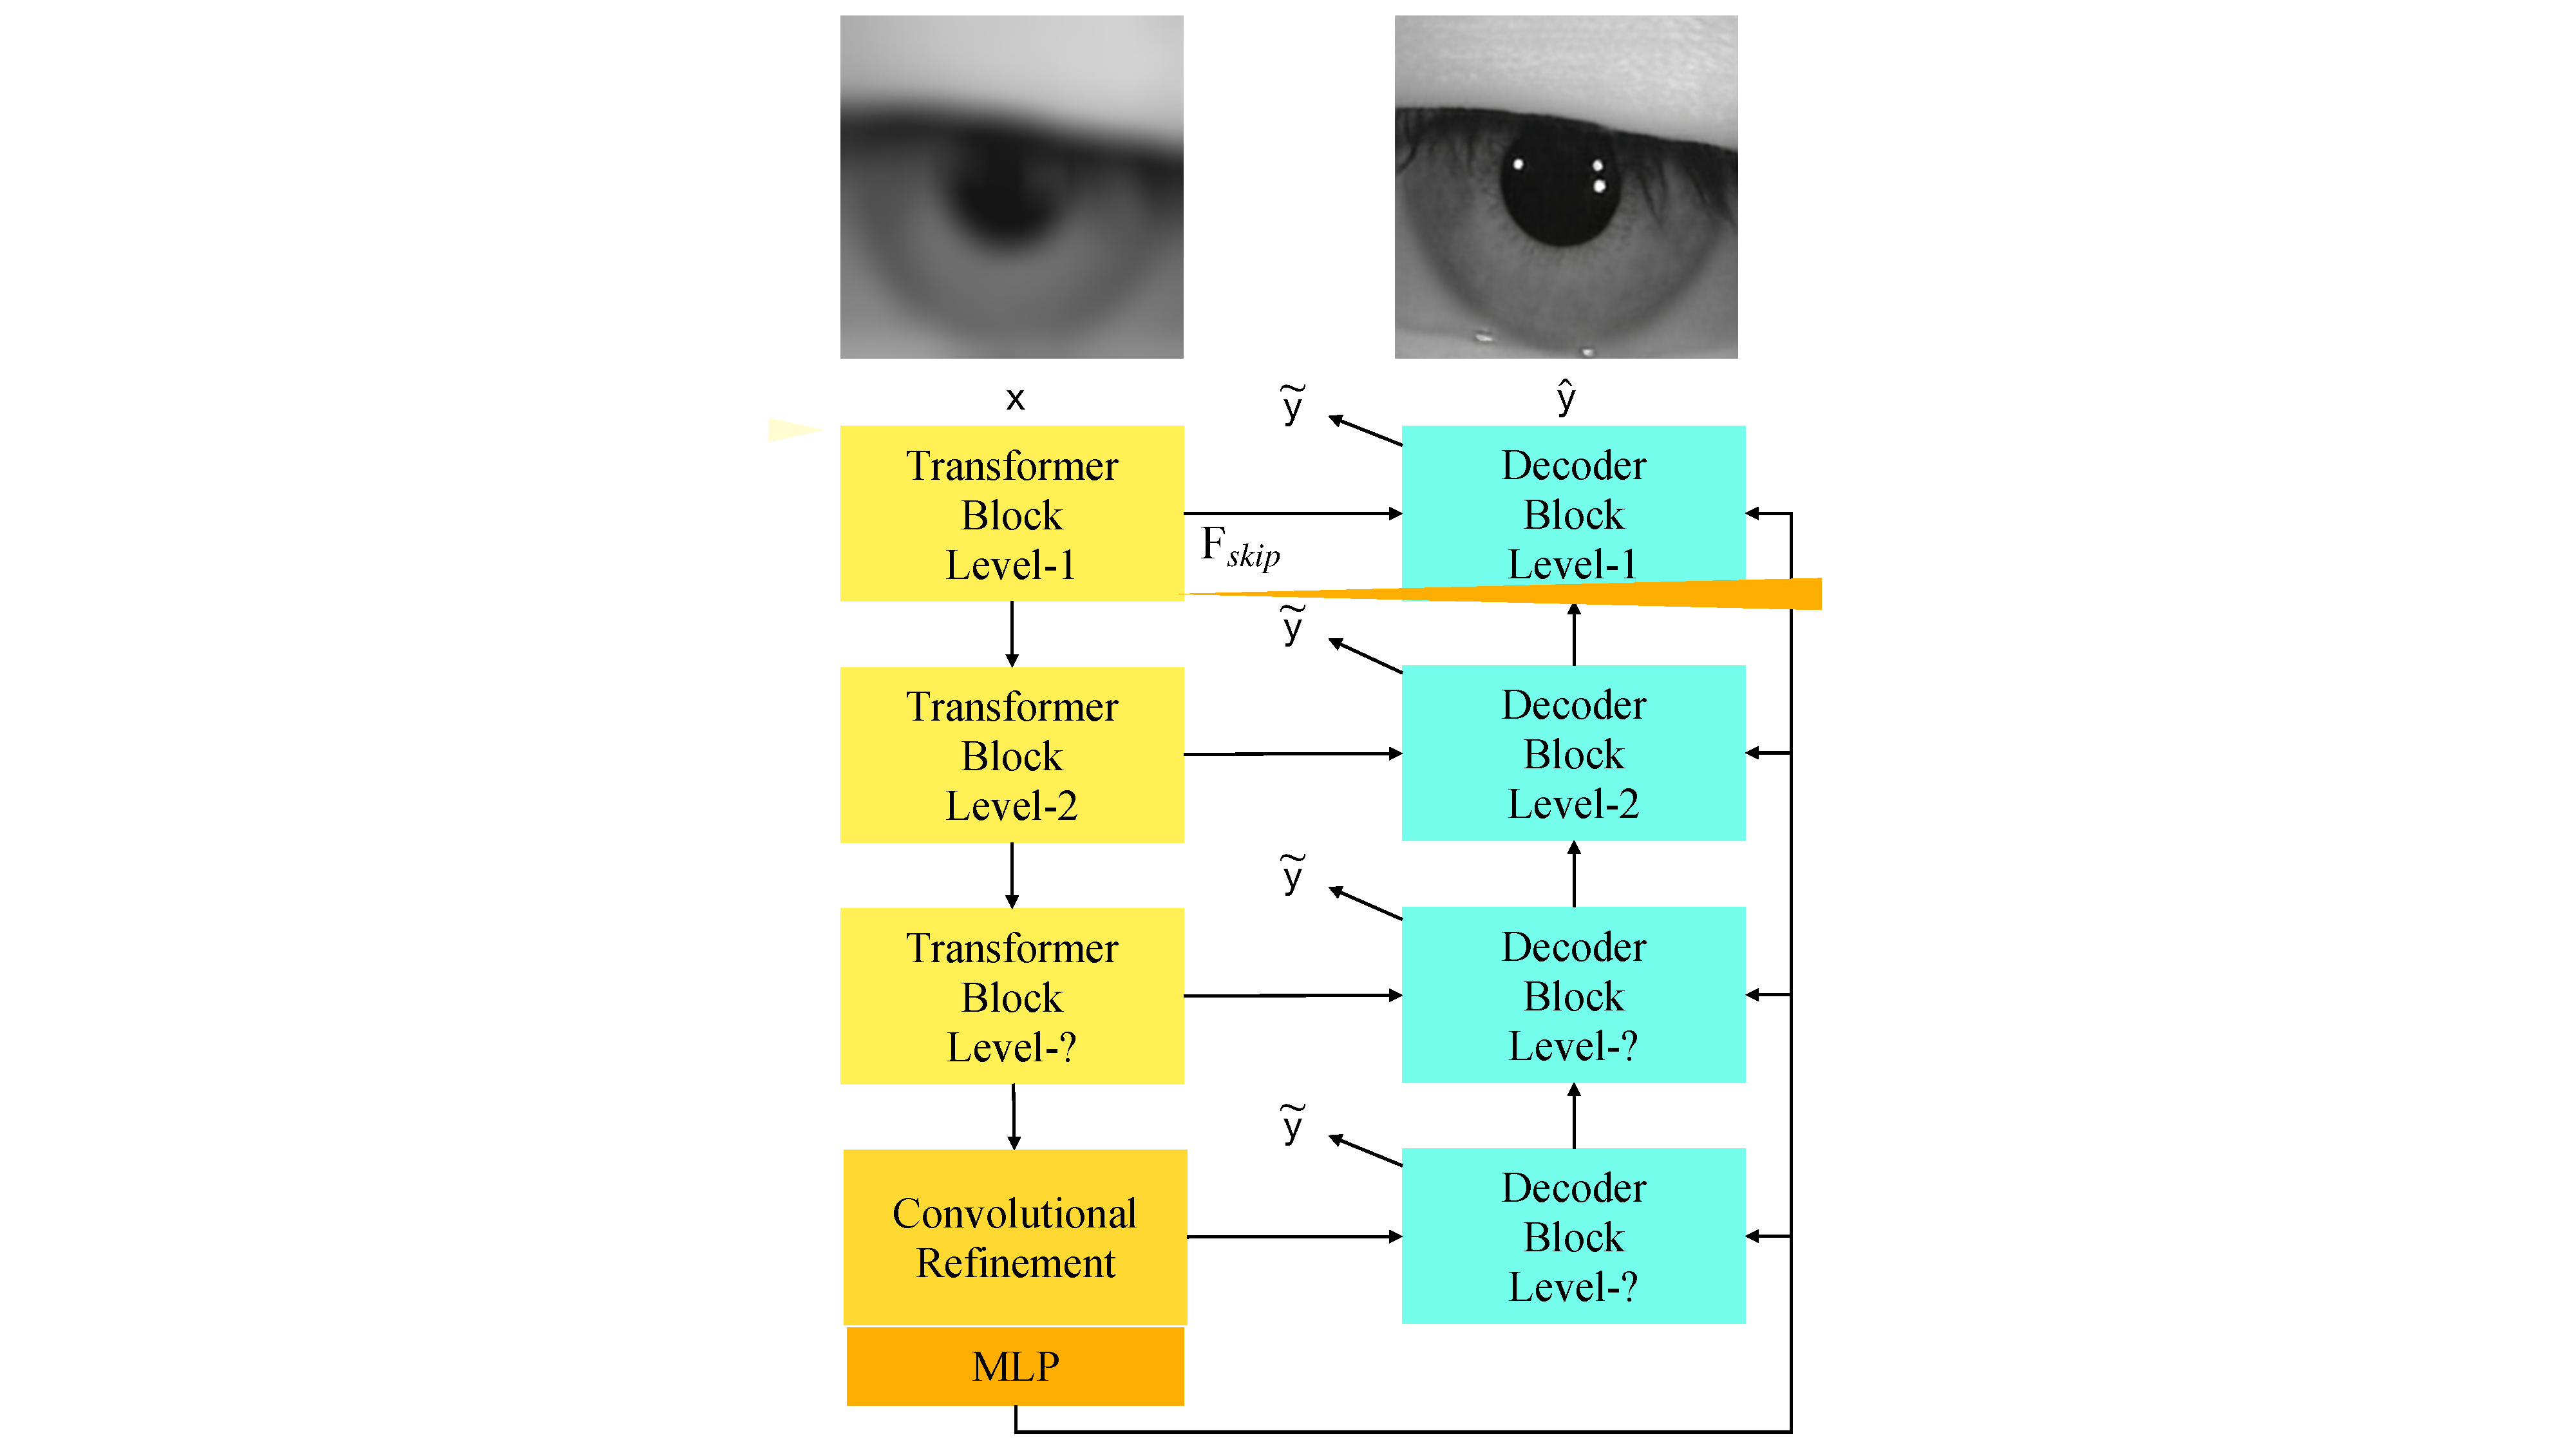
\includegraphics[width=4.5cm]{chanel1.pdf}
	\end{textblock*}		

\end{frame}


%------------------------------------------------

\subsubsection{实验配置与结果}

\begin{frame}
	\frametitle{实验数据}
	\framesubtitle{} % Optional subtitle
	\begin{varblock}[0.55\textwidth]{}
		\small 本文使用了
		\begin{enumerate}
			\item 灯
			\item 千人数据集
		\end{enumerate}			
	\end{varblock}	

	\begin{textblock*}{6cm}(9.5cm,2.2cm) % {block width} (coords)
		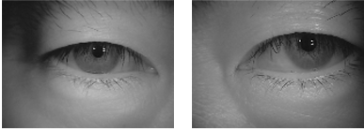
\includegraphics[width=6cm]{lamp.png}
	\end{textblock*}	
	\begin{textblock*}{6cm}(9.5cm,5.4cm) % {block width} (coords)
		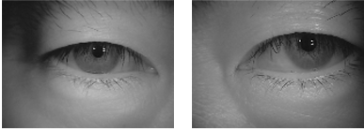
\includegraphics[width=6cm]{lamp.png}
	\end{textblock*}	
\end{frame}

%------------------------------------------------

\begin{frame}
	\frametitle{定量实验结果}
	\framesubtitle{} % Optional subtitle
	
	\begin{table}
	\footnotesize
\begin{tabular}{ccc ccc ccc}
  \hline
  % after \\: \hline or \cline{col1-col2} \cline{col3-col4} ...
Method & FFF $\uparrow$ & GGG $\downarrow$	& \makecell{HHH \\ =0.001 $\uparrow$} & \makecell{III \\ =0.01 $\uparrow$} & JJJ $\uparrow$ & KKK $\uparrow$ & LLL $\downarrow$ \\ \hline
输入 & 9521 & 1153 & 1992 & 5361 & 368 & 8336 & 2865 \\
AAAA & 9796 & 0705 & 5356 & 7538 & \textbf{34.15} & \textbf{8808} & 1249 \\
BBBB & 9818 & 0679 & 5608 & 7666 & 33.57 & 8789 & 1324 \\
CCCC & 9732 & 0853	& 3960 & 6705 & 32.85 & 8695 & 1311 \\
DDDD & 9585	& 1093 & 4816 & 6876 & 329 & 8314 & \textbf{1189} \\
EEEE & 9836 & 0542 & 5878 & 8274 & 32.36 & 8729 & 1350 \\
\alert{本章方法} & \alert{9864} & \alert{0532} & \alert{7475} & \alert{8773} & 32.82 & 8754 & 1513 \\
 \hline
原始图像 & 9914 & 0274 & 9323& 9613 & - & - & -\\ \hline
\end{tabular}
		\caption{方法1与现有方法的定量结果对比。}
	\end{table}
\end{frame}


%------------------------------------------------

\subsection{方法2}

\subsubsection{理论分析}

\begin{frame}
	\frametitle{\large 方法2}
	\framesubtitle{\normalsize 骨干网络} % Optional subtitle
	\begin{varblock}[0.7\textwidth]{}
		\small 生成
	\end{varblock}	
	\begin{varblock}[0.7\textwidth]{}
		\small 工作。
	\end{varblock}	
	\begin{varblock}[0.7\textwidth]{}
		\small 解码器
	\end{varblock}		
	\begin{textblock*}{4.5cm}(11.2cm,1.8cm) % {block width} (coords)
		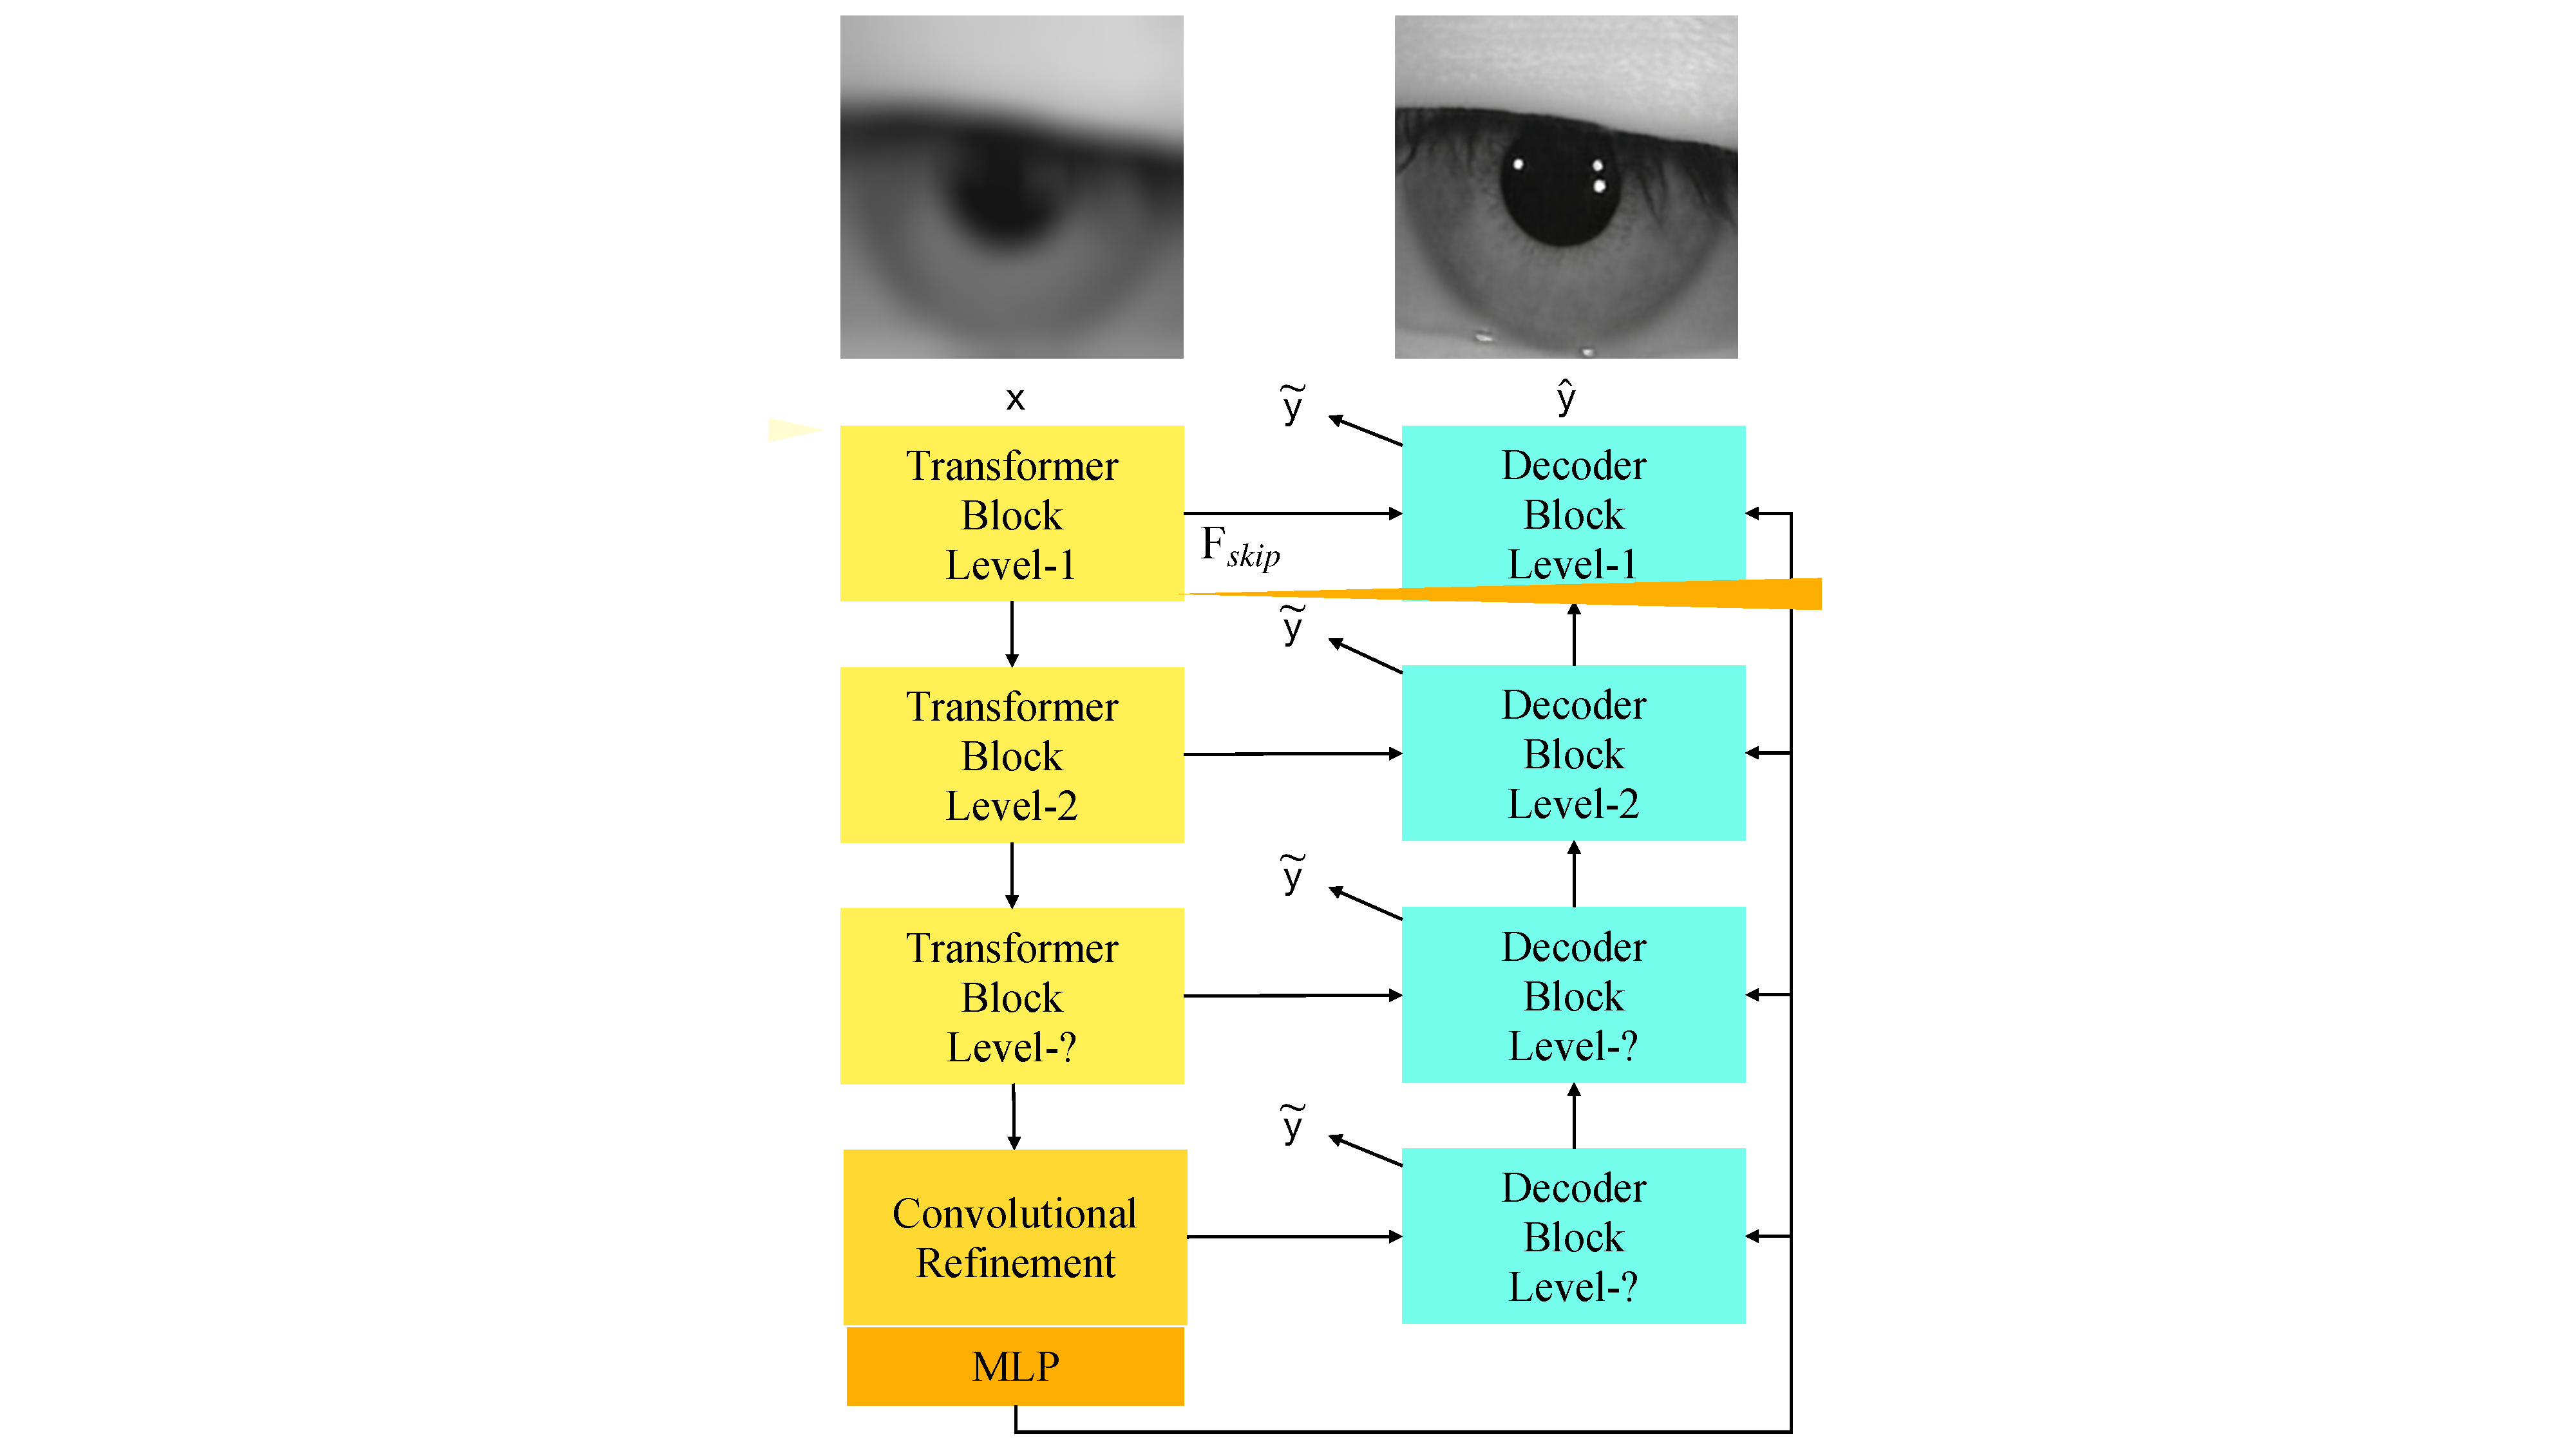
\includegraphics[width=4.5cm]{chanel1.pdf}
	\end{textblock*}		

\end{frame}

%------------------------------------------------

\subsubsection{实验配置与结果}

%------------------------------------------------

\begin{frame}
	\frametitle{\large 方法2}
	\framesubtitle{\normalsize 实验设置} % Optional subtitle
	\begin{varblock}[0.65\textwidth]{}
		\begin{itemize}
			\item 实验数据
			\item 采用的
			\item Adam
			\item 深度学习框架为PyTorch。
			\item GPU型号
		\end{itemize}	
	\end{varblock}	

	\begin{textblock*}{5.5cm}(10.5cm,2cm) % {block width} (coords)
		
\includegraphics[width=5.5cm]{pytorch.jpg}
	\end{textblock*}	
	\begin{textblock*}{4cm}(11cm,4cm) % {block width} (coords)
		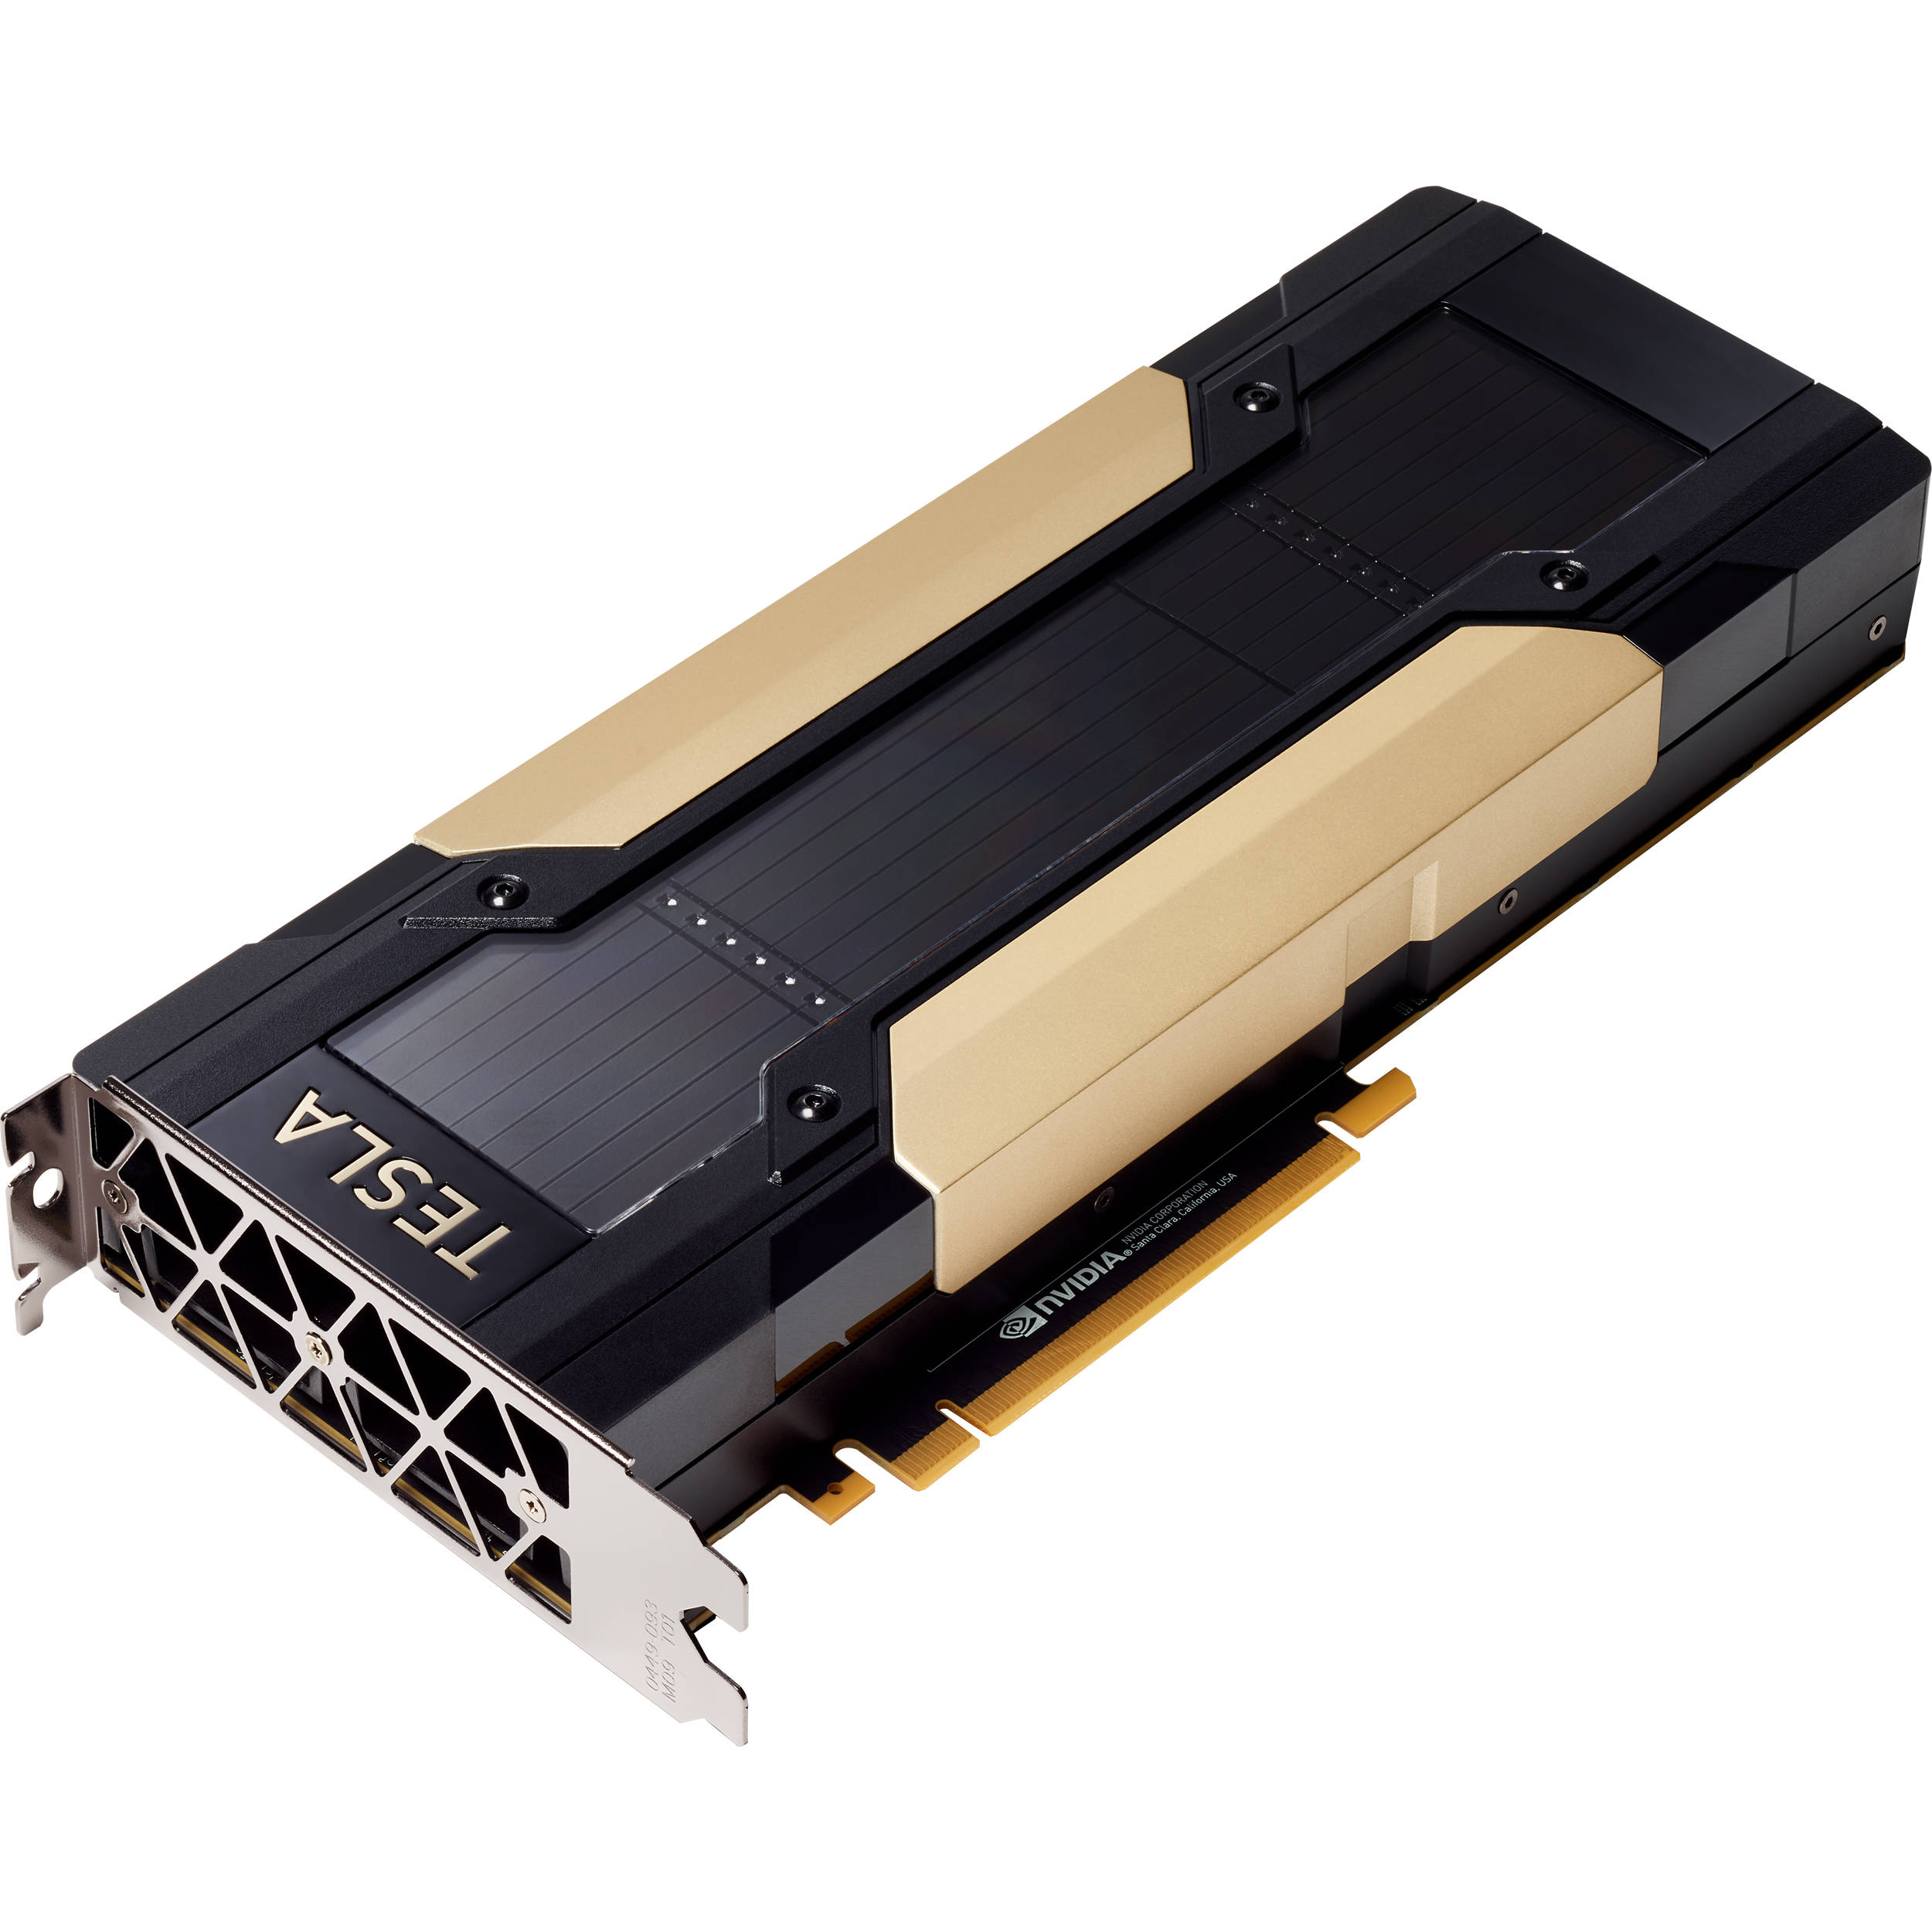
\includegraphics[width=4cm]{v100.jpg}
	\end{textblock*}	

\end{frame}


%------------------------------------------------

\begin{frame}
	\frametitle{消融实验}
	\framesubtitle{} % Optional subtitle
	
	\begin{table}
	\footnotesize
\begin{tabular}{ccc ccc ccc}
  \hline
  % after \\: \hline or \cline{col1-col2} \cline{col3-col4} ...
Method & DDD $\uparrow$ & EEE $\downarrow$	& \makecell{FFF \\ =0.01 $\uparrow$} & \makecell{GGG \\ =1 $\uparrow$} & HHH $\uparrow$ & III $\uparrow$ \\ \hline
w/o AAA & 9513 & 1273 & 5145 & 6678 & 29.43 & 8023  \\
w/o BBB & 9903 & 0435 & 7889 & 9060 & 32.96 & 8734  \\
w/o CCC & 9879 & 0480 & 7721 & 8917 & 32.12 & 8582  \\
本章方法 & 9883 & 0505 & 7843 & 0.8873 & 32.88 & 0.8631 \\ \hline
\end{tabular}
		\caption{方法2的消融实验结果。}
	\end{table}
\end{frame}

%------------------------------------------------

\section{总结与展望}

\begin{frame}
	\frametitle{工作总结}
	\begin{varblock}[1\textwidth]{}
		\small 	传统自注意力机制
	\end{varblock}		
	\begin{varblock}[1\textwidth]{}
		\small 	传统的	\end{varblock}				
	\begin{varblock}[1\textwidth]{}
		\small 	传统的	
	\end{varblock}		
\end{frame}

%------------------------------------------------

\begin{frame}
	\frametitle{工作展望}
	\begin{varblock}[1\textwidth]{}
	 	\small 本文的方法中	
	\end{varblock}		
	
	\begin{varblock}[1\textwidth]{}
%		\setstretch{1}
	 	\small 本文的方法中
	\end{varblock}		
				
	\begin{varblock}[1\textwidth]{}
	 	\small 本文的方法
	\end{varblock}	
	

\end{frame}
%------------------------------------------------

\begin{frame}
	\frametitle{攻读学位期间发表的学术论文}
[1]
\end{frame}


%----------------------------------------------------------------------------------------
%	CLOSING SLIDE
%----------------------------------------------------------------------------------------

\begin{frame}[plain] % The optional argument 'plain' hides the headline and footline
	\begin{center}
		{\Huge \textbf{谢谢}}
		
		\bigskip\bigskip % Vertical whitespace
		
		{\LARGE 欢迎各位老师指正!}
	\end{center}
\end{frame}

%----------------------------------------------------------------------------------------

\end{document} 